
\subsection{An Example of Test Path and Input Generation}

\begin{figure*}[htb]
%\begin{figure*}[!b]
  \centering
  \begin{minipage}[t]{0.31\textwidth}
    \centering
    \lstset{language=PHP, title=v0.php (original version),
basicstyle=\footnotesize,  tabsize=2}
    \lstinputlisting{figures/v0.php}
  \end{minipage}
  \begin{minipage}[t]{0.31\textwidth}
   \lstset{language=PHP, title=v1.php (modified version),
basicstyle=\footnotesize, tabsize=2}
    \lstinputlisting{figures/v1.php}
  \end{minipage}
    \begin{minipage}[t]{0.35\textwidth}
      \caption*{\\PDG for v0 and v1}
      \vspace*{6pt}
    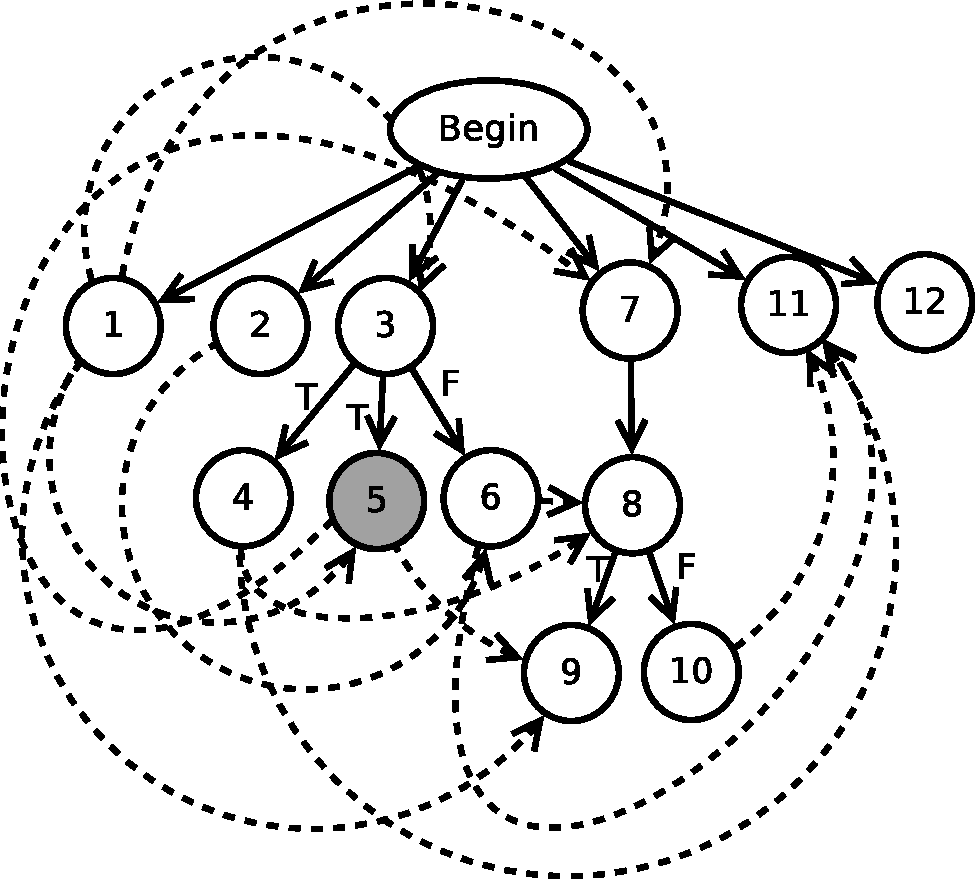
\includegraphics[width=\textwidth]{figures/flow2.pdf}

  \end{minipage}
  \caption{Path Generation Example Program}
%\vspace*{-5pt}
  \label{fig:example}
\end{figure*}



We illustrate how we generate test paths using program slices.
Suppose we have a simple PHP program (v0.php) and its 
modified program (v1.php) as shown in Figure \ref{fig:example}.
The rightmost graph shows a PDG for v0.php and v1.php.

In the PDG, the solid lines represent control dependence edges, 
and the dashed lines represent data dependence edges. 
As the example shows, statement 5 has changed, so our slicing
algorithm takes node 5 and variable $a$ ($<$5, $a>$) as a slicing 
criterion. By performing forward and backward slicing, the slice 
with respect to $<$5, $a>$ includes nodes 1, 5, 7, and 9 (node 1 
from backward slicing, and nodes 7 and 9 from forward slicing). 

Having obtained this slice, the path generator creates subpaths 
starting from the first node in it (in this example, node 1). 
As the tool walks the path using control flow information, 
it adds nodes 2 and 3 to a subpath (\{1, 2, 3\}). 
Once the path generator reaches node 3, it has a choice to 
explore one of the control successors (4 and 6).
When the tool analyzes the path containing edge 
3 $\rightarrow$ 4, it sees that the next 
control successor is node 5, yielding a subpath of 
\{1, 2, 3, 4, 5\}. 
When the tool analyzes the path containing edge 
3 $\rightarrow$ 6, it discovers that
there is no path from node 6 to node 5. It then discards
path \{1, 2, 3, 6\}. 
 
Continuing with the remaining edges, the tool produces
a subpath of \{1, 2, 3, 4, 5, 7, 8\}. Because node 8 
is another branching node, the tool yields subpaths 
\{1, 2, 3, 4, 5, 7, 8, 9\} and \{1, 2, 3, 4, 5, 7, 8, 10\}. 
Edges 8 $\rightarrow$ 9 and 8 $\rightarrow$ 10 are marked as 
covered by the path generator. The tool then recognizes that 
subpath \{1, 2, 3, 4, 5, 7, 8, 10\} ends with a node that is 
outside the impact set. (It is impossible to go from node 10 
back to nodes \{1, 5, 7, 9\}.) The tool also recognizes that 
there is no path from node 7 to node 9 that goes through node 10. 
The tool then discards this path. This process is repeated until 
all nodes in a slice have been visited.

Having generated subpaths that contain all nodes in a slice,
the tool walks the program dependence graph from the 
first node to the beginning of the program (In this case, node 1 
is at the beginning.) and walks the last node in the path to the 
end of the program by adding nodes 11 and 12 to it.
In this example, the tool generates one final path,
\{1, 2, 3, 4, 5, 7, 8, 9, 11, 12\}.
Note that, without applying our approach, we need to generate
four linearly independent paths to test the modified program,
v1.php. 

The next step is to generate inputs for the created path. 
First, the constraint collector gathers constraint information
by analyzing all the path's branching nodes. 
In our example for path \{1, 2, 3, 4, 5, 7, 8, 9, 11, 12\}, 
three constraints are collected:  
\$ POST[`inputA'] $<$ 12 , \$ POST[`inputA']-3 $>$ 7, and 
\$ POST[`inputB'] $==$ 5. 
Using a constraint solver, we can choose input values 11 and 
5 for \$ POST[`inputA'] and \$ POST[`inputB'], respectively.
Once these values are resolved, the test execution engine
can simply use them as inputs for the web application to walk 
the desired path.

 
